\documentclass[aspectratio=169]{beamer}

\usepackage{graphicx}
\usepackage{minted}
\usepackage{subcaption}

\usetheme{firedrake}

\title{Two more tiny Python packages for scientific computing: mpi-pytest and petsctools}
\author{Connor Ward}
\date{07/07/2025}

\begin{document}

\frame{\titlepage}

% some little tools that I maintain that the community may be interested in
% they might be niche so I just want a little bit of your time

\begin{frame}{About me}
  \begin{itemize}
    \item
      I work on the Firedrake finite element framework
    \item
      I write a lot of Python
    \item
      I work with HPC + MPI
  \end{itemize}
\end{frame}

% As well as FEM, Firedrake solved mini problems that non-Firedrake people
% want. Historically people have needed to copy the code like this.
\begin{frame}{Motivation}
  \centering

  \vspace{-2em}

  \begin{minipage}{.8\textwidth}
    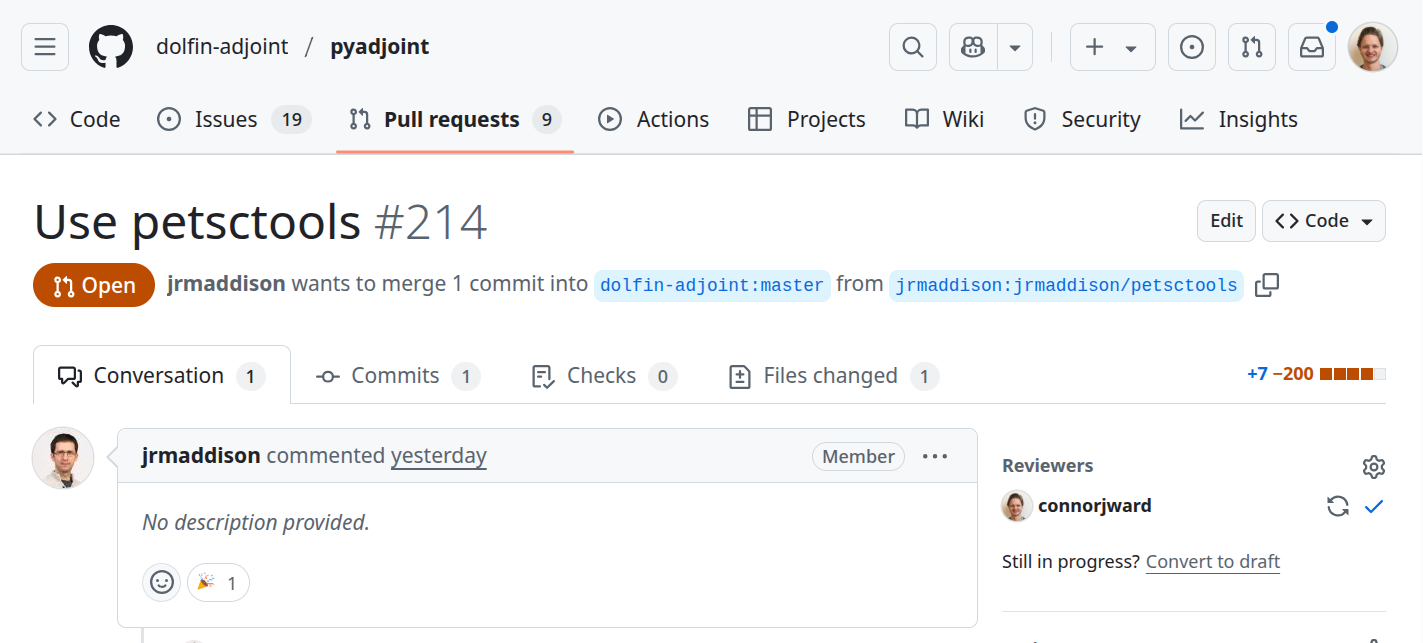
\includegraphics[width=\textwidth]{figures/petsctools_pr.png}
  \end{minipage}

  \vspace{1em}

  \begin{minipage}{.8\textwidth}
    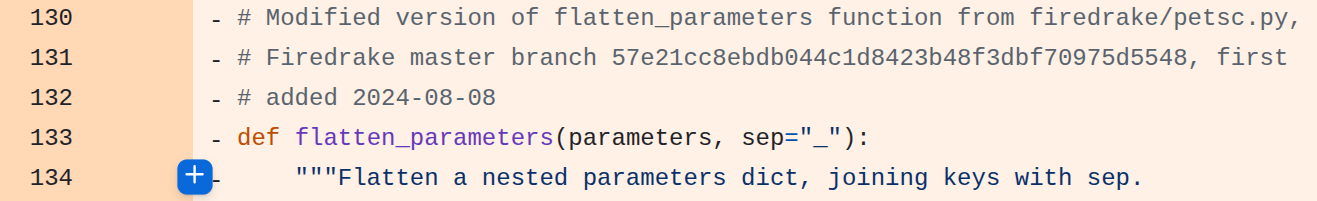
\includegraphics[width=\textwidth]{figures/dead_comment.png}
  \end{minipage}
\end{frame}

\begin{frame}[t,fragile]{mpi-pytest}
  \vspace{3em}

  \begin{columns}
    \begin{column}{.4\textwidth}
      \begin{minted}[fontsize=\tiny,autogobble=true]{python}

        def test_comm_world_size_equals_two():
          assert COMM_WORLD.size == 2



        def test_comm_world_size_equals_three():
          assert COMM_WORLD.size == 3
      \end{minted}
    \end{column}
    \begin{column}{.6\textwidth}
      \begin{minted}[fontsize=\tiny,autogobble=true]{bash}
        $ pytest test_comms.py  # won't work!

        $ mpiexec -n 2 pytest test_comms.py  # won't work!
      \end{minted}
    \end{column}
  \end{columns}
\end{frame}

\begin{frame}[t,fragile]{mpi-pytest}
  \vspace{3em}

  \begin{columns}
    \begin{column}{.4\textwidth}
      \begin{minted}[fontsize=\tiny,autogobble=true,highlightlines={1,6},highlightcolor=red!30]{python}
        @pytest.mark.parallel(2)
        def test_comm_world_size_equals_two():
          assert COMM_WORLD.size == 2


        @pytest.mark.parallel(3)
        def test_comm_world_size_equals_three():
          assert COMM_WORLD.size == 3
      \end{minted}
    \end{column}
    \begin{column}{.6\textwidth}
      \begin{minted}[fontsize=\tiny,autogobble=true]{bash}
        $ pytest test_comms.py  # works, calls MPI under the hood

        $ mpiexec -n 2 pytest test_comms.py -m parallel[2]  # works
      \end{minted}
    \end{column}
  \end{columns}

  \vspace{2em}

  \pause

  \begin{center}
    \footnotesize{\texttt{pip install mpi-pytest}}
  \end{center}
\end{frame}

\begin{frame}{petsctools}
  \begin{itemize}
    \item
      PETSc's Python bindings (petsc4py) mimic the C API
    \item
      petsctools provides `Pythonic extensions'
  \end{itemize}

  \pause

  Examples include:

  \begin{itemize}
    \item
      Managing nested trees of options
    \item
      Reading PETSc configuration information
    \item
      (TODO) Custom monitors (e.g. plot convergence)
    \item
      (TODO) Passing data between Python and PETSc
    \item
      And more...
  \end{itemize}

  \pause

  \centering{
    \footnotesize{\texttt{pip install petsctools}}
  }
\end{frame}

\end{document}
